\documentclass[addpoints]{exam}

\usepackage{epic,array,ecltree,url, calrsfs}
\usepackage[nointegrals]{wasysym}
\usepackage{mlextra}


%These tell TeX which packages to use.
\usepackage{epsfig}
\usepackage{amsmath}
\usepackage{amsfonts}
\usepackage{amssymb}
\usepackage{amsxtra}
\usepackage{amsthm}
\usepackage{mathrsfs}
\usepackage[dvipsnames]{xcolor}
\usepackage{array}
\usepackage{graphicx}
\graphicspath{ {../art/} }
\usepackage{bm}
\usepackage{tikz}
\usepackage{multicol}

\renewcommand\qedsymbol{$\blacksquare$}

%Here I define some theorem styles and shortcut commands for symbols I use often
\theoremstyle{definition}
\newtheorem{defn}{Definition}
\newtheorem{thm}{Theorem}
\newtheorem{cor}{Corollary}
\newtheorem*{rmk}{Remark}
\newtheorem{lem}{Lemma}
\newtheorem*{joke}{Joke}
\newtheorem{ex}{Example}
\newtheorem*{soln}{Solution}
\newtheorem{prop}{Proposition}

\newcommand{\lra}{\longrightarrow}
\newcommand{\ra}{\rightarrow}
\newcommand{\surj}{\twoheadrightarrow}
\newcommand{\graph}{\mathrm{graph}}
\newcommand{\bb}[1]{\mathbb{#1}}
\newcommand{\Ell}{\mathscr{L}}
\newcommand{\Z}{\bb{Z}}
\newcommand{\Q}{\bb{Q}}
\newcommand{\R}{\bb{R}}
\newcommand{\C}{\bb{C}}
\newcommand{\N}{\bb{N}}
\newcommand{\M}{\mathbf{M}}
\newcommand{\m}{\mathbf{m}}
\newcommand{\MM}{\mathscr{M}}
\newcommand{\HH}{\mathscr{H}}
\newcommand{\Om}{\Omega}
\newcommand{\Ho}{\in\HH(\Om)}
\newcommand{\bd}{\partial}
\newcommand{\del}{\partial}
\newcommand{\bardel}{\overline\partial}
\newcommand{\textdf}[1]{\textbf{\textsf{#1}}\index{#1}}
\newcommand{\img}{\mathrm{img}}
\newcommand{\ip}[2]{\left\langle{#1},{#2}\right\rangle}
\newcommand{\inter}[1]{\mathrm{int}{#1}}
\newcommand{\exter}[1]{\mathrm{ext}{#1}}
\newcommand{\cl}[1]{\mathrm{cl}{#1}}
\newcommand{\ds}{\displaystyle}
\newcommand{\vol}{\mathrm{vol}}
\newcommand{\cnt}{\mathrm{ct}}
\newcommand{\osc}{\mathrm{osc}}
\newcommand{\LL}{\mathbf{L}}
\newcommand{\UU}{\mathbf{U}}
\newcommand{\support}{\mathrm{support}}
\newcommand{\AND}{\;\wedge\;}
\newcommand{\OR}{\;\vee\;}
\newcommand{\Oset}{\varnothing}
\newcommand{\st}{\ni}
\newcommand{\wh}{\widehat}

\newcommand{\id}[1]{\mbox{\it #1\/}}
\newcommand{\rid}[1]{\mbox{\rm #1}}
\newcommand{\sid}[1]{\mbox{\sf #1}}
\newcommand{\bid}[1]{\mbox{\bf #1}}
\newcommand{\tinysz}[1]{\mbox{\tiny $#1$}}

%Pagination stuff.
\setlength{\topmargin}{-.3 in}
\setlength{\oddsidemargin}{0in}
\setlength{\evensidemargin}{0in}
\setlength{\textheight}{9.in}
\setlength{\textwidth}{6.5in}



%\pagestyle{empty} 
%\footer{}{\thepage}{}

\newcommand{\twonode}{%
  \begingroup\normalfont
  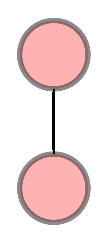
\includegraphics[height=\fontcharht\font`\b]{2nodetree.eps}%
  \endgroup
}

\newcommand{\tf}[1][{}]{%
\fillin[#1][0.25in]%
}
\noprintanswers
\unframedsolutions
\SolutionEmphasis{\itshape\small}
\SolutionEmphasis{\color{NavyBlue}}
\checkboxchar{$\Box$}
\checkedchar{$\blacksquare$}
\begin{document}


\noindent
\begin{tabular*}{\textwidth}{l @{\extracolsep{\fill}} r @{\extracolsep{6pt}} l}
{\large CS3920: Foundations of Computer Science} &  \makebox[3in]{\large Name:\enspace\hrulefill}\\
{\large May 29, 2018} & \\
{\large Quiz 4} & 
\end{tabular*}\\

\fbox{\fbox{\parbox{6in}{\textbf{Instructions}: Please answer the questions 
  below to the best of your ability. Be sure to show your work where appropriate. 
   This quiz is closed book, closed notes, closed computer. There are \numpoints\ 
   points in total. }}}\\
\begin{questions}
\question[2] Let $A$ and $B$ be two problems such that $A$ reduces to $B$. Which of
the following can you conclude (choose all that apply)?
\begin{checkboxes}
\CorrectChoice If $A$ is NP-complete, $B$ is NP-Hard.
\CorrectChoice $B$ is at least as hard as $A$.
\CorrectChoice If $B$ is decidable, $A$ is also decidable.
\choice If $A$ is in $P$, $B$ is in NP. 
\end{checkboxes}

\vspace{5mm}
\question Evaluate the formula $A$ under the interpretation given.
\begin{parts}
\part[1] \tf[T] (T/F) $A = \forall x \exists y p(x,y) \imp \exists x \forall y
    p(x,y)$ and $\mathcal{I}_A = (\Z,\{<\},\{\})$
%\part[1] \tf[T] (T/F) $A = \exists x (p(x) \land \exists x q(x) \implies \exists x
%    (p(x) \land q(x))$ and $\mathcal{I}_A = (\{1,2\},\{\{1\},\{2\}\},\{\})$
\vspace{5mm}
\part[1] \tf[T] (T/F) $A = \forall x \forall y (p(x,y) \imp p(f(x,a), f(y,a)))$
and $\mathcal{I}_A = (\Z,\{\{ = \}\},\{\{+\}\},\{0\})$
\end{parts}
\vspace{5mm}

\question[3] Let $S$ be a propositional logic formula in clausal form, such that $S =
\{s,\bar{r}s, \bar{s}\bar{r}\bar{t}, rt\}$. Use DPLL to find a satisfying interpretation. 
Draw the execution tree. 


\end{questions}
\end{document}


